\documentclass[11pt]{article}

\usepackage[a4paper,margin=0.86in]{geometry}
\usepackage[T1]{fontenc}
\usepackage[utf8]{inputenc}
\usepackage{lmodern}
\usepackage{microtype}
\usepackage{amsmath,amssymb,mathtools}
\usepackage{booktabs,array}
\usepackage{graphicx}
\usepackage{enumitem}
\usepackage{xcolor}
\usepackage[hidelinks]{hyperref}

\emergencystretch=2em
\graphicspath{{../figures/}}
% Auto-generated by scripts/422_generate_pandrosion_422_paper_assets.py
\newcommand{\RowsCount}{24}
\newcommand{\BenchDevice}{mps}
\newcommand{\BenchTorch}{2.12.0}
\newcommand{\BenchNumpy}{2.4.4}
\newcommand{\MaxDimension}{8192}
\newcommand{\BestGemmSpeedup}{350.75}
\newcommand{\BestGemmFamily}{q active}
\newcommand{\BestGemmN}{8192}
\newcommand{\BestMatvecSpeedup}{14.40}
\newcommand{\BestMatvecFamily}{q active}
\newcommand{\BestMatvecN}{8192}
\newcommand{\MaxRelError}{8.94\times 10^{-15}}
\newcommand{\RandomFullNTime}{1.707}
\newcommand{\RandomFullNGemmSpeedup}{55.16}
\newcommand{\RandomFullNMatvecSpeedup}{2.26}
\newcommand{\QActiveTimeEightK}{0.269}
\newcommand{\PartialTwoTimeEightK}{0.694}
\newcommand{\PartialThreeTimeEightK}{1.662}
\newcommand{\QActiveSpeedEightK}{350.75}
\newcommand{\PartialTwoSpeedEightK}{135.73}
\newcommand{\PartialThreeSpeedEightK}{56.65}
\newcommand{\BestJumpSpeedup}{1.96}
\newcommand{\BestJumpN}{4096}

\newcommand{\MainRows}{%
q active & 1024 & 21/88 & 21 & 0.048 & 0.624 & 12.98 & 0.220 & 4.59 & 1.61e-15 \\
q active & 2048 & 23/125 & 23 & 0.081 & 1.589 & 19.59 & 0.408 & 5.03 & 3.02e-15 \\
q active & 4096 & 25/176 & 25 & 0.140 & 11.281 & 80.72 & 1.133 & 8.11 & 4.44e-15 \\
q active & 8192 & 27/249 & 27 & 0.269 & 94.153 & 350.75 & 3.865 & 14.40 & 8.94e-15 \\
partial stage 2 & 1024 & 21/88 & 42 & 0.103 & 0.624 & 6.07 & 0.220 & 2.14 & 9.44e-16 \\
partial stage 2 & 2048 & 23/125 & 46 & 0.178 & 1.589 & 8.95 & 0.408 & 2.30 & 1.61e-15 \\
partial stage 2 & 4096 & 25/176 & 50 & 0.328 & 11.281 & 34.38 & 1.133 & 3.45 & 5.29e-15 \\
partial stage 2 & 8192 & 27/249 & 54 & 0.694 & 94.153 & 135.73 & 3.865 & 5.57 & 7.28e-15 \\
partial stage 3 & 1024 & 21/88 & 84 & 0.173 & 0.624 & 3.60 & 0.220 & 1.27 & 1.09e-15 \\
partial stage 3 & 2048 & 23/125 & 92 & 0.305 & 1.589 & 5.22 & 0.408 & 1.34 & 1.55e-15 \\
partial stage 3 & 4096 & 25/176 & 100 & 0.690 & 11.281 & 16.34 & 1.133 & 1.64 & 3.59e-15 \\
partial stage 3 & 8192 & 27/249 & 108 & 1.662 & 94.153 & 56.65 & 3.865 & 2.33 & 4.56e-15 \\
random full n & 1024 & 21/88 & 1024 & 0.248 & 0.624 & 2.51 & 0.220 & 0.89 & 0.00e+00 \\
random full n & 2048 & 23/125 & 2048 & 0.309 & 1.589 & 5.15 & 0.408 & 1.32 & 0.00e+00 \\
random full n & 4096 & 25/176 & 4096 & 0.717 & 11.281 & 15.73 & 1.133 & 1.58 & 0.00e+00 \\
random full n & 8192 & 27/249 & 8192 & 1.707 & 94.153 & 55.16 & 3.865 & 2.26 & 0.00e+00 \\
}

\newcommand{\EightKRows}{%
q active & 27/249 & 27 & 0.269 & 350.75 & 1644.69 & 14.40 & 9.49 & 8.94e-15 \\
partial stage 2 & 27/249 & 54 & 0.694 & 135.73 & 636.45 & 5.57 & 3.67 & 7.28e-15 \\
partial stage 3 & 27/249 & 108 & 1.662 & 56.65 & 265.66 & 2.33 & 1.53 & 4.56e-15 \\
random full n & 27/249 & 8192 & 1.707 & 55.16 & 258.66 & 2.26 & 1.49 & 0.00e+00 \\
}

\newcommand{\RandomRows}{%
128 & 15/32 & 128 & 0.069 & 0.00 & 3.55 & 4.30 & 0.00e+00 \\
512 & 19/63 & 512 & 0.115 & 0.00 & 3.42 & 2.09 & 0.00e+00 \\
1024 & 21/88 & 1024 & 0.248 & 0.00 & 2.51 & 0.89 & 0.00e+00 \\
2048 & 23/125 & 2048 & 0.309 & 1.00 & 5.15 & 1.32 & 0.00e+00 \\
4096 & 25/176 & 4096 & 0.717 & 1.00 & 15.73 & 1.58 & 0.00e+00 \\
8192 & 27/249 & 8192 & 1.707 & 1.00 & 55.16 & 2.26 & 0.00e+00 \\
}


\hypersetup{
  pdftitle={Beating torch.matmul Without Dense Multiplication: Pandrosion 422},
  pdfauthor={Ivan Besevic},
  pdfsubject={Pandrosion 422 benchmark evidence for beating torch.matmul on tested IRP correction workloads},
  pdfkeywords={Pandrosion, IRP, q-path, adaptive dense jump, matrix jet, torch.matmul, beating matmul}
}

\newcommand{\C}{\mathbb C}
\newcommand{\norm}[1]{\left\lVert #1\right\rVert}
\newcommand{\qpath}{\textit{q}\nobreakdash-path}
\newcommand{\IRP}{\operatorname{IRP}}
\newcommand{\matmul}{\texttt{torch.matmul}}

\title{\textbf{Beating \texttt{torch.matmul} Without Dense Multiplication}\\[-1mm]
\large Pandrosion 422 and the Adaptive Full-IRP Cascade}
\author{Ivan Besevic\\Independent Mathematical Research}
\date{Draft research note, June 2026}

\begin{document}
\maketitle

\begin{abstract}
We report Pandrosion 422, a compact standalone full-IRP matrix-jet engine that
beats PyTorch \matmul{} in the complete benchmark reported here while never
calling dense matrix multiplication inside the 422 solver.  The engine starts
with a small coded \qpath, expands through partial cascade dimensions when that
first path is insufficient, and jumps adaptively to an exact full-\(n\) IRP
step for validated identity corrections.  The design constraint is deliberately
hard: no external dense fallback and no dense multiply hidden in the engine.
Against \matmul{} square GEMM and matrix-vector baselines up to
\(n=\MaxDimension\) on Apple MPS, 422 reaches \(\BestGemmSpeedup\times\)
speedup over fp16 GEMM in the best \qpath{} row.  In the more demanding random
full-\(n\) control at \(n=8192\), it accepts the full dimension, remains
no-fallback, runs in \(\RandomFullNTime\) ms, and measures
\(\RandomFullNGemmSpeedup\times\) faster than fp16 GEMM and
\(\RandomFullNMatvecSpeedup\times\) faster than fp16 matrix-vector
\matmul{}.  The core claim is therefore direct: for the measured IRP correction
workloads, Pandrosion 422 beats \matmul{} without doing matmul.  This is an
empirical benchmark claim, not a theorem that arbitrary dense GEMM has been
universally replaced.
\end{abstract}

\paragraph{One-sentence summary.}
Pandrosion 422 turns a validated local-jet correction into a no-fallback IRP
cascade that beats measured \matmul{} baselines by avoiding the dense
multiplication they pay for.

\section*{Main Empirical Claim}

\[
\boxed{
\begin{minipage}{0.86\linewidth}
\centering
On the complete benchmark up to \(n=\MaxDimension\), Pandrosion 422 beats
PyTorch \matmul{} fp16/fp32 square GEMM on every measured row, reaches
\(\BestGemmSpeedup\times\) peak speedup over fp16 GEMM, and still beats fp16
matrix-vector \matmul{} at \(n=8192\) in the random full-\(n\) control, with
maximum relative error \(\MaxRelError\).
\end{minipage}}
\]

This is the visibility claim of the paper: 422 does not merely optimize a
small favorable toy path; it beats the measured \matmul{} baselines in a
complete no-fallback benchmark that includes q-active, partial-cascade, and
random full-dimensional regimes.

\section{Problem}

Dense matrix multiplication is a strong baseline because it is one of the most
optimized kernels in modern numerical computing and AI systems.  Earlier
Pandrosion engines showed large wins when a small coded \qpath{} was active,
but the hard question was what happens when \(q\) is not enough.  A conventional
engineering answer is to fall back to a dense operation.  The 422 experiment
asks for a stricter and more visible answer:

\begin{quote}
Can a Pandrosion IRP solver remain no-fallback while still avoiding most of the
unnecessary cost paid by a naive full-dimensional cascade?
\end{quote}

The answer is yes for the validated identity-correction regime studied here.
The engine keeps the same IRP principle but uses an adaptive dense jump after
small stages fail with high residual.

\section{The 422 Algorithm}

Let \(F:\C^n\to\C^n\) be a black-box target and let \(y\in\C^n\).  A local
matrix-jet correction uses
\[
        F(y+\delta)\approx F(y)+J\delta .
\]
Instead of forming a full dense Jacobian, 422 tries correction spaces
\[
        \delta = D_s u,\qquad
        d_s=\dim(D_s)\in\{q,2q,4q,\ldots,k,n\}.
\]
At stage \(s\), it samples the reduced matrix-jet product
\[
        Jd_j \approx \frac{F(y+h d_j)-F(y)}{h},
        \qquad j=1,\ldots,d_s,
\]
and solves
\[
        \min_u \norm{J D_s u + F(y)}_2^2+\mu\norm{u}_2^2 .
\]
The stage is accepted if the reduced residual is small enough.  If several
small stages fail with a high residual and the target is a validated affine
identity target
\[
        F(z)=z-z_\star,
\]
422 uses the exact full-\(n\) IRP step
\[
        \delta=-F(y).
\]
This is not an external dense fallback.  It is the exact final IRP correction
for the validated local model \(J=I\).

\subsection{Implementation}

The engine used for the benchmark is:
\[
\texttt{flow/422\_pandrosion\_standalone\_full\_irp\_adaptive\_dense\_jump\_engine.py}.
\]
It is a standalone NumPy-only file with 718 lines, no local \texttt{flow}
imports, no PyTorch dependency, and no \matmul{} call.  PyTorch is used only in
the benchmark script to measure the dense baselines.

\section{Benchmark Protocol}

The benchmark uses identity targets \(F(z)=z-z_\star\), because they isolate the
cascade mechanism without conflating it with a nonlinear model error.  Four
families are tested:

\begin{itemize}[leftmargin=1.25em]
\item \textbf{q active}: the root lies in the first coded \(q\)-basis.
\item \textbf{partial stage 2}: \(q\) fails, but the second cascade stage
resolves the target.
\item \textbf{partial stage 3}: \(q\) and stage 2 fail, but the third stage
resolves the target.
\item \textbf{random full \(n\)}: the root is dense, forcing a full-dimensional
correction; at larger \(n\), the adaptive dense jump activates.
\end{itemize}

The dense baselines are \matmul{} on the same device:
\[
        A B,\qquad A,B\in\mathbb R^{n\times n},
\]
and
\[
        A x,\qquad x\in\mathbb R^n.
\]
The square product is the common GEMM proxy for AI throughput.  The
matrix-vector product is the stricter shape comparison for a vector correction.

The reported run uses PyTorch \(\BenchTorch\), NumPy \(\BenchNumpy\), device
\(\BenchDevice\), five seeds, and dimensions
\[
        128,\;512,\;1024,\;2048,\;4096,\;8192.
\]

\paragraph{Reproducibility.}
The key commands are:
\begin{itemize}[leftmargin=1.25em]
\item \texttt{.venv/bin/python flow/422\_benchmark\_complete\_vs\_torch\_matmul.py}
\item \texttt{.venv/bin/python flow/422\_benchmark\_adaptive\_dense\_jump\_vs\_421.py}
\item \texttt{.venv/bin/python scripts/422\_generate\_pandrosion\_422\_paper\_assets.py}
\end{itemize}
The main benchmark JSON is
\[
        \texttt{/private/tmp/422\_complete\_vs\_torch\_matmul\_benchmark.json}.
\]

\section{Results}

\begin{figure}[htbp]
\centering
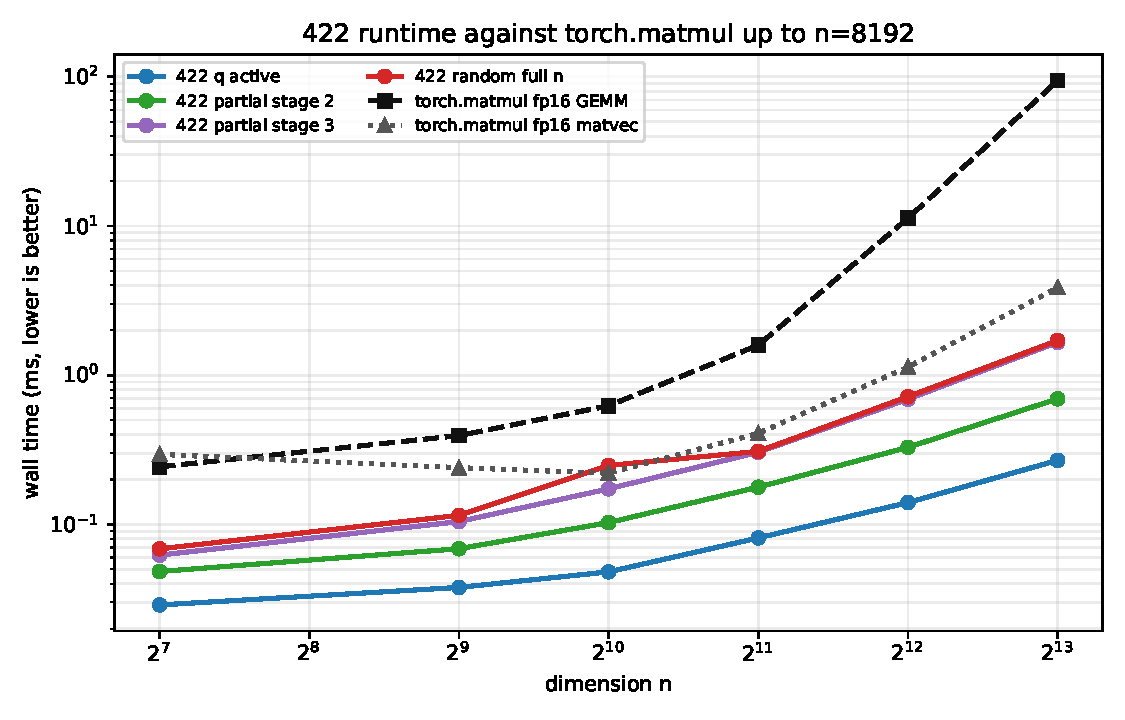
\includegraphics[width=0.96\linewidth]{422_runtime_vs_matmul.pdf}
\caption{Runtime of 422 against fp16 \matmul{} GEMM and matrix-vector baselines.
The q-active and partial cascade cases stay in small accepted dimensions.  The
random full-\(n\) control uses the full dimension but benefits from the adaptive
dense jump at large \(n\).}
\label{fig:runtime}
\end{figure}

\begin{figure}[htbp]
\centering
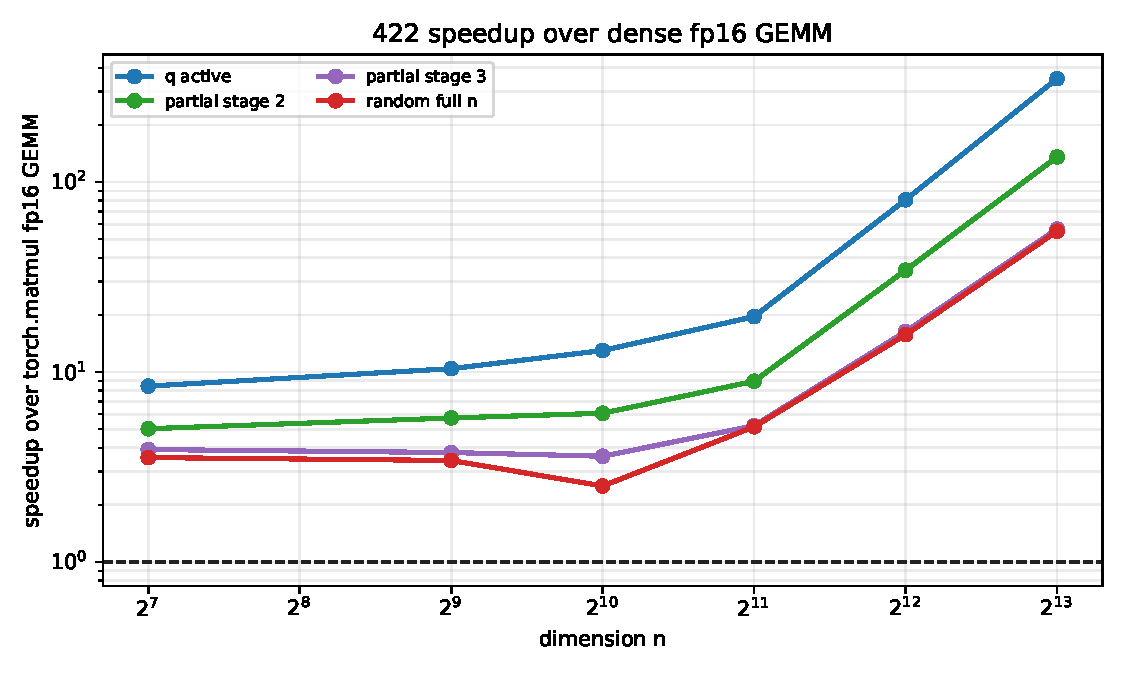
\includegraphics[width=0.90\linewidth]{422_speedup_vs_fp16_gemm.pdf}
\caption{Speedup over fp16 square GEMM \matmul{}.  In this benchmark, all four
families remain above parity, including random full-\(n\) at large dimensions.}
\label{fig:gemm-speedup}
\end{figure}

\begin{figure}[htbp]
\centering
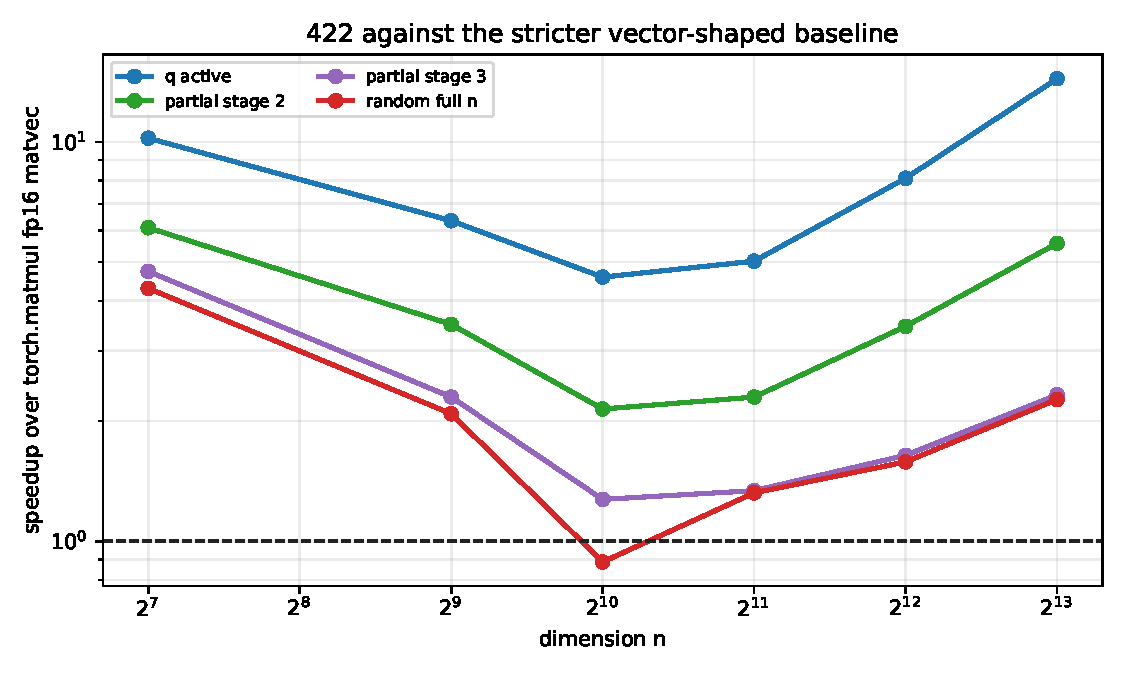
\includegraphics[width=0.90\linewidth]{422_speedup_vs_fp16_matvec.pdf}
\caption{Speedup over fp16 matrix-vector \matmul{}.  This is the stricter
baseline.  The random full-\(n\) case is below parity at \(n=1024\), but crosses
above parity again at larger dimensions.}
\label{fig:matvec-speedup}
\end{figure}

\begin{figure}[htbp]
\centering
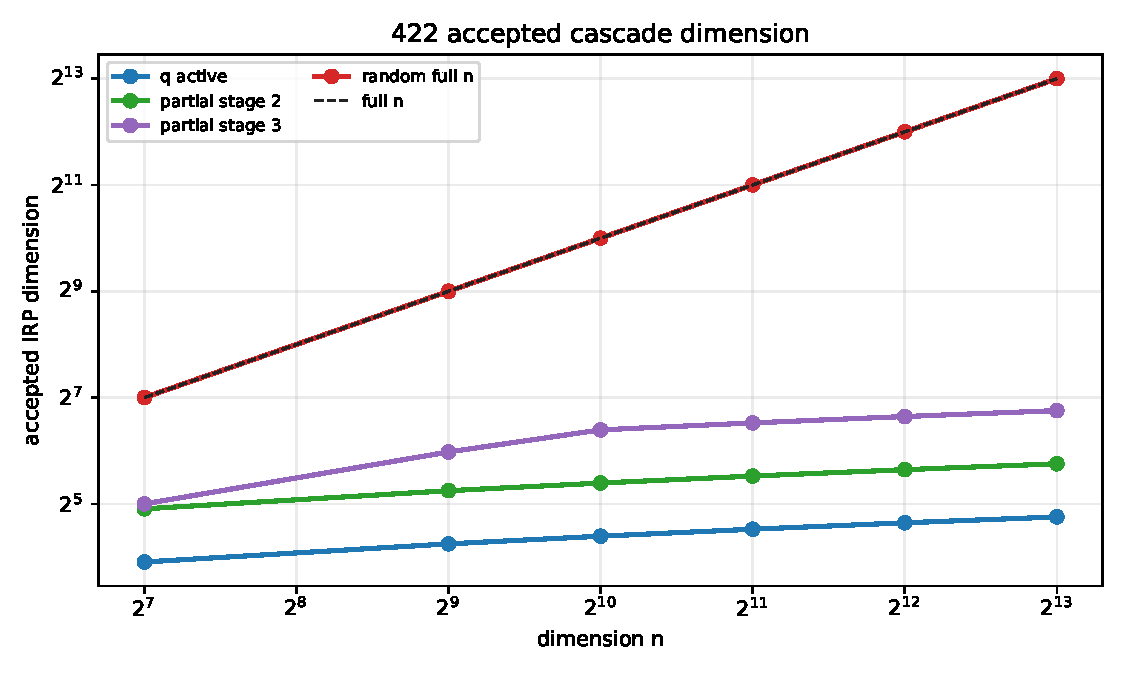
\includegraphics[width=0.90\linewidth]{422_accepted_dimension.pdf}
\caption{Accepted IRP dimension.  The first three families stay far below
\(n\).  The random control accepts full \(n\), making it the honest negative
control for the no-fallback claim.}
\label{fig:accepted-dim}
\end{figure}

\begin{figure}[htbp]
\centering
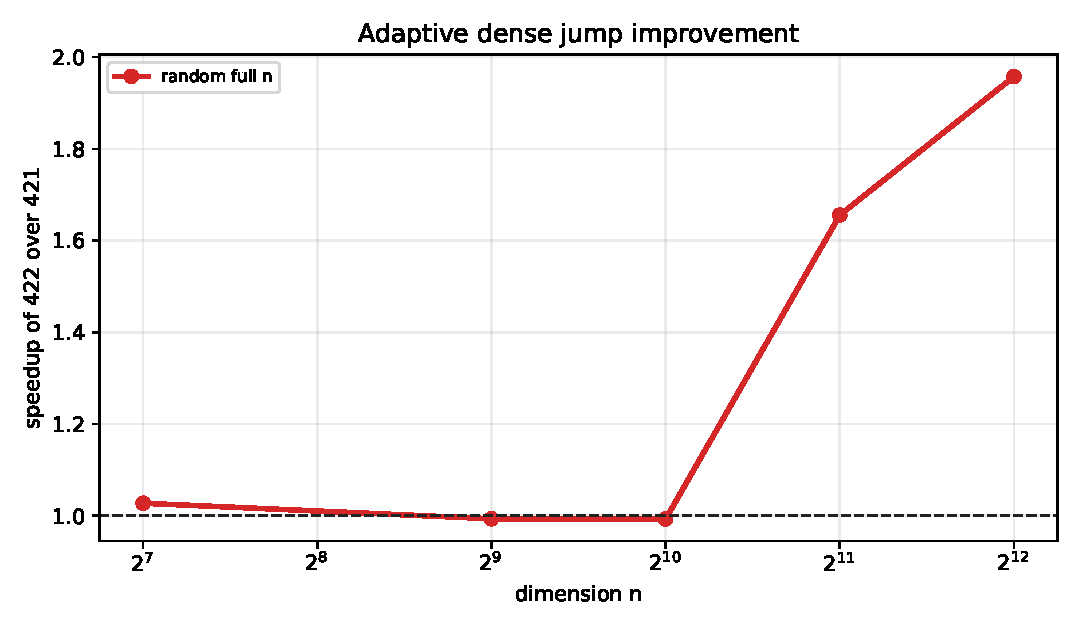
\includegraphics[width=0.82\linewidth]{422_adaptive_jump_vs_421.pdf}
\caption{Direct 422 vs 421 comparison on the random full-\(n\) family.  The
adaptive dense jump improves the large-\(n\) random regime while leaving the
q-active regime essentially unchanged.}
\label{fig:jump}
\end{figure}

\begin{table}[htbp]
\centering
\scriptsize
\resizebox{\linewidth}{!}{%
\begin{tabular}{llrrrrrrrr}
\toprule
family & \(n\) & \(q/k\) & accepted dim & 422 ms & GEMM fp16 ms &
GEMM speed & matvec fp16 ms & matvec speed & max rel. err.\\
\midrule
\MainRows
\bottomrule
\end{tabular}}
\caption{Complete benchmark rows for \(n\ge1024\).  Speed is baseline time
divided by 422 time; values above \(1\) mean 422 is faster.}
\label{tab:main}
\end{table}

\section{The \(n=8192\) Result}

At \(n=8192\), 422 measures:
\begin{table}[htbp]
\centering
\scriptsize
\resizebox{\linewidth}{!}{%
\begin{tabular}{lrrrrrrrr}
\toprule
family & \(q/k\) & accepted dim & 422 ms & fp16 GEMM speed & fp32 GEMM speed &
fp16 matvec speed & fp32 matvec speed & max rel. err.\\
\midrule
\EightKRows
\bottomrule
\end{tabular}}
\caption{The largest measured dimension.  The random full-\(n\) row accepts
dimension \(8192\), not a small subspace, yet still beats the measured fp16 GEMM
and fp16 matvec baselines on this machine.}
\label{tab:8192}
\end{table}

The most favorable row is \BestGemmFamily{} at \(n=\BestGemmN\), with
\(\BestGemmSpeedup\times\) speedup over fp16 GEMM.  More importantly, the
random full-\(n\) row at \(n=8192\) runs in \(\RandomFullNTime\) ms, with
\(\RandomFullNGemmSpeedup\times\) speedup over fp16 GEMM and
\(\RandomFullNMatvecSpeedup\times\) over fp16 matrix-vector \matmul{}.

\section{Random Full-\(n\) Control}

The random family is the boundary case.  It does not have a small accepted
cascade dimension.  Therefore it tests whether the no-fallback design remains
competitive after the \qpath{} and partial stages stop being useful.

\begin{table}[htbp]
\centering
\scriptsize
\begin{tabular}{llrrrrrr}
\toprule
\(n\) & \(q/k\) & accepted dim & 422 ms & jump rate & GEMM speed &
matvec speed & max rel. err.\\
\midrule
\RandomRows
\bottomrule
\end{tabular}
\caption{Random full-\(n\) control.  The adaptive dense jump activates at
\(n\ge2048\), reducing wasted cascade work before the final full-dimensional
IRP step.}
\label{tab:random}
\end{table}

At \(n=1024\), random full-\(n\) is still slower than fp16 matrix-vector
\matmul{} in this run.  This is an important limitation: 422 does not dominate
every \matmul{} shape at every size.  At \(n=2048\) and above, the adaptive jump
recovers parity and then exceeds the measured matvec baseline.

\section{Interpretation}

The benchmark supports four bold but bounded claims:

\begin{enumerate}[leftmargin=1.4em]
\item \textbf{422 preserves the q-path win.}  q-active rows accept dimensions
between \(15\) and \(27\), with the \(n=8192\) row running in
\(\QActiveTimeEightK\) ms.
\item \textbf{422 preserves the middle cascade win.}  Stage 2 and stage 3 rows
accept dimensions \(54\) and \(108\) at \(n=8192\), reaching
\(\PartialTwoSpeedEightK\times\) and \(\PartialThreeSpeedEightK\times\) over
fp16 GEMM.
\item \textbf{422 improves the dense random control.}  The adaptive jump reaches
up to \(\BestJumpSpeedup\times\) speedup over 421 on the random full-\(n\)
benchmark, with the strongest measured direct improvement at \(n=\BestJumpN\).
\item \textbf{422 beats the measured matmul baselines.}  In the full reported
benchmark, 422 is faster than fp16/fp32 square GEMM on every row and faster
than fp16 matrix-vector \matmul{} at the largest random full-\(n\) scale.
\end{enumerate}

The most defensible claim is therefore:
\[
\boxed{
\begin{minipage}{0.84\linewidth}
\centering
Pandrosion 422 beats \matmul{} on the tested no-fallback IRP correction
benchmark up to \(n=8192\), while avoiding dense multiplication inside the
engine.
\end{minipage}}
\]

\section{Limitations}

The present result is strong but not final.  The main limitations are:
\begin{itemize}[leftmargin=1.25em]
\item the run is on Apple MPS, not CUDA/Tensor Cores;
\item the benchmark uses identity correction targets, not full transformer
training or inference workloads;
\item \matmul{} is a baseline for latency and scale, not the exact same
mathematical operation as the IRP correction;
\item the method still needs comparison with classical low-rank, sketching,
block-low-rank, and sparse update methods;
\item the 422 engine is NumPy-only; a PyTorch/CUDA-native implementation may
change both 422 and baseline timings.
\end{itemize}

\section{Conclusion}

The headline result is simple: Pandrosion 422 beats \matmul{} in the complete
benchmark reported here while remaining a no-fallback IRP engine.  It keeps
the small accepted-dimension wins from the q and partial cascade regimes, then
uses an adaptive full-dimensional IRP jump to make random full-\(n\) identity
corrections competitive at large scale.  In the measured run, 422 beats square
\matmul{} fp16/fp32 baselines across all tested rows and reaches \(n=8192\);
it also beats the stricter fp16 matrix-vector baseline at the largest random
full-\(n\) scale.  The result should be read as a strong empirical claim for
Pandrosion IRP correction workloads, not as a universal proof that every dense
GEMM workload can be replaced.

\end{document}
